% TransFusionHead detail (heatmap-guided query init + transformer decoder).
\documentclass[tikz,border=8pt]{standalone}
% Shared styles for the DSB architecture diagrams.
\usepackage[T1]{fontenc}
\usepackage{graphicx}
\usetikzlibrary{arrows.meta, backgrounds, calc, fit, positioning, shapes.geometric}

\definecolor{camA}{HTML}{2A78D6}
\definecolor{lidA}{HTML}{1BAF7A}
\definecolor{fusA}{HTML}{EB6834}
\definecolor{detA}{HTML}{6250D6}
\definecolor{segA}{HTML}{0E8FA8}
\definecolor{occA}{HTML}{B5482A}
\definecolor{inkA}{HTML}{262626}
\definecolor{mutA}{HTML}{6B6B6B}

\tikzset{
  blk/.style={
    draw=inkA!70, line width=0.45pt, rounded corners=2.5pt,
    align=center, font=\small, inner sep=3pt,
    minimum height=0.95cm, text=inkA, fill=white,
  },
  cam/.style={blk, fill=camA!10, draw=camA!75},
  lid/.style={blk, fill=lidA!10, draw=lidA!75},
  fus/.style={blk, fill=fusA!12, draw=fusA!80},
  det/.style={blk, fill=detA!10, draw=detA!75},
  seg/.style={blk, fill=segA!10, draw=segA!75},
  occ/.style={blk, fill=occA!10, draw=occA!75},
  io/.style={blk, fill=black!4, draw=inkA!55},
  arr/.style={-{Stealth[length=2.2mm,width=1.6mm]}, line width=0.65pt, draw=inkA!75},
  darr/.style={arr, dashed},
  tag/.style={font=\scriptsize, text=mutA},
  grp/.style={draw=mutA!70, dashed, line width=0.6pt, rounded corners=6pt, inner sep=8pt},
  hdr/.style={font=\normalsize\bfseries, text=inkA, anchor=west},
  note/.style={font=\scriptsize, text=mutA, align=left},
}


\begin{document}
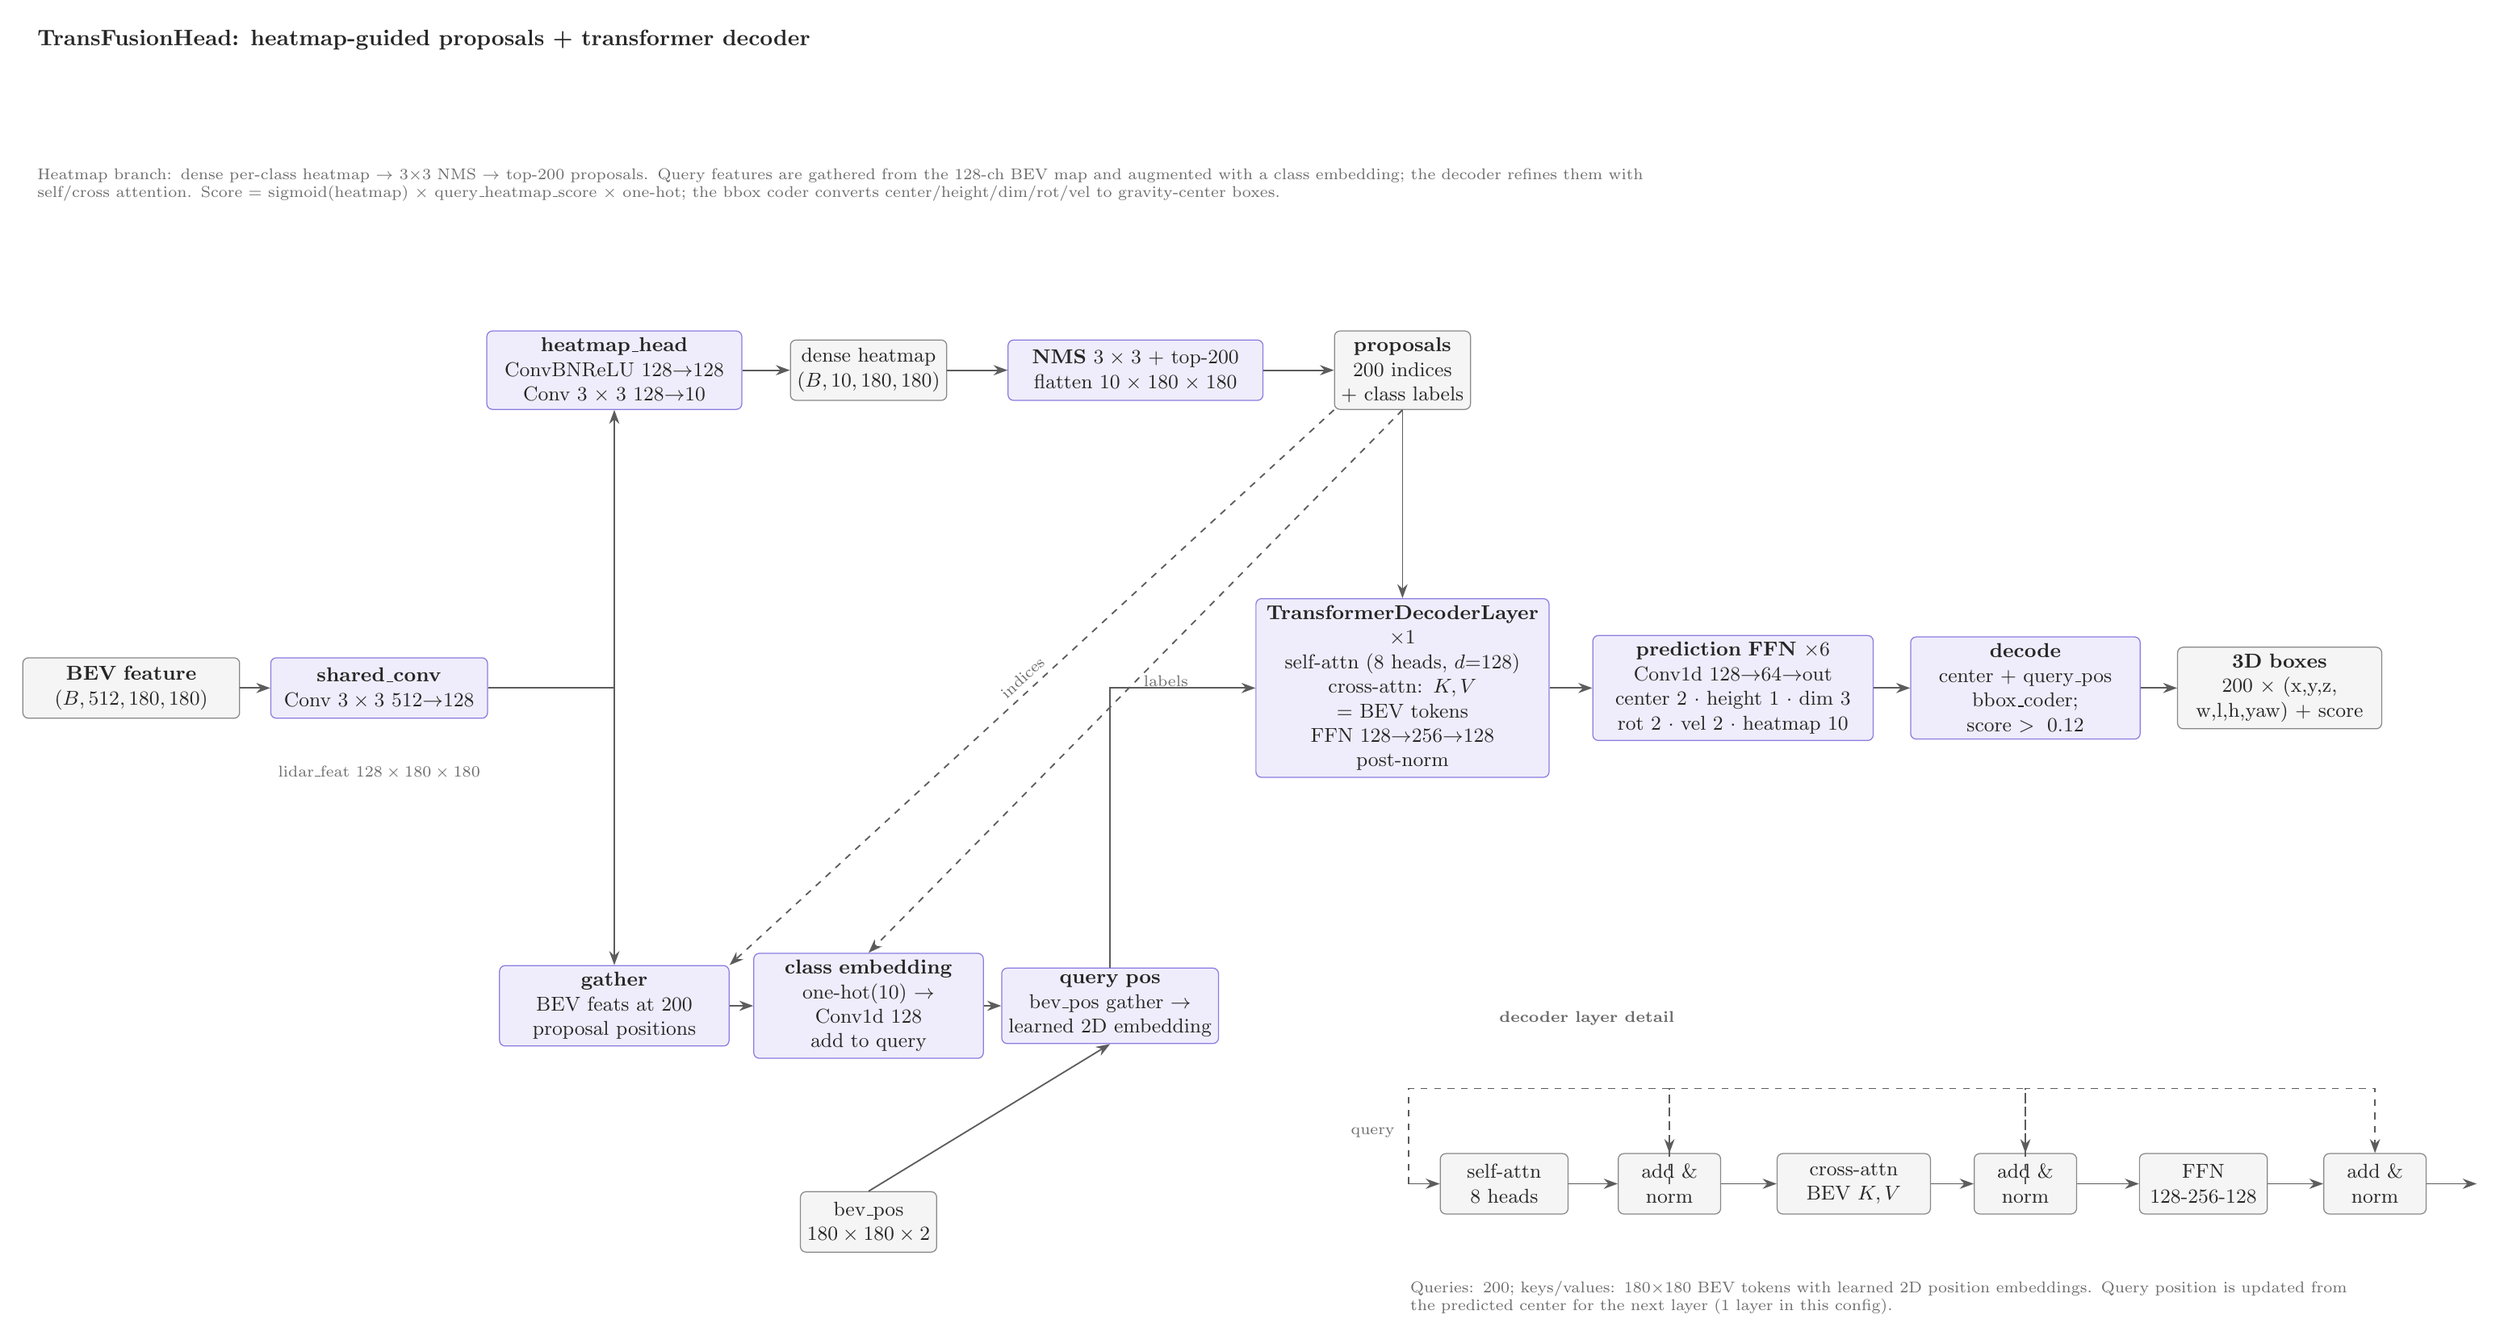
\begin{tikzpicture}

% ---------------------------------------------------------------- shared trunk
\node[io, text width=3.2cm] (bev) at (0,12)
  {\textbf{BEV feature}\\$(B,512,180,180)$};
\node[det, text width=3.2cm] (shared) at (3.9,12)
  {\textbf{shared\_conv}\\Conv $3\times3$ 512$\to$128};
\draw[arr] (bev) -- (shared);
\node[tag, anchor=north] at (3.9,10.9) {lidar\_feat $128\times180\times180$};

% ---------------------------------------------------------------- heatmap branch
\node[det, text width=3.8cm] (hh) at (7.6,17)
  {\textbf{heatmap\_head}\\ConvBNReLU 128$\to$128\\
   Conv $3\times3$ 128$\to$10};
\node[io] (dense) at (11.6,17) {dense heatmap\\$(B,10,180,180)$};
\node[det, text width=3.8cm] (nms) at (15.8,17)
  {\textbf{NMS} $3\times3$ + top-200\\flatten $10\times180\times180$};
\node[io] (prop) at (20.0,17)
  {\textbf{proposals}\\200 indices\\+ class labels};

\draw[arr] (shared.east) -| (hh.south);
\draw[arr] (hh) -- (dense);
\draw[arr] (dense) -- (nms);
\draw[arr] (nms) -- (prop);

% ---------------------------------------------------------------- query init
\node[det, text width=3.4cm] (gather) at (7.6,7)
  {\textbf{gather}\\BEV feats at 200\\proposal positions};
\node[det, text width=3.4cm] (cls) at (11.6,7)
  {\textbf{class embedding}\\one-hot(10) $\to$ Conv1d 128\\
   add to query};
\node[det, text width=3.2cm] (qpos) at (15.4,7)
  {\textbf{query pos}\\bev\_pos gather $\to$\\
   learned 2D embedding};
\node[io] (bevpos) at (11.6,3.6) {bev\_pos\\$180\times180\times2$};

\draw[arr] (shared.east) -| (gather.north);
\draw[arr] (gather) -- (cls);
\draw[arr] (cls) -- (qpos);
\draw[arr] (bevpos.north) -- (qpos.south);
\draw[arr, dashed] (prop.south west) -- (gather.north east)
  node[midway, above, tag, sloped] {indices};
\draw[arr, dashed] (prop.south) -- (cls.north)
  node[midway, right, tag] {labels};

% ---------------------------------------------------------------- decoder
\node[det, text width=4.4cm] (decoder) at (20.0,12)
  {\textbf{TransformerDecoderLayer} $\times1$\\self-attn (8 heads, $d$=128)\\
   cross-attn: $K,V$ = BEV tokens\\FFN 128$\to$256$\to$128\\post-norm};
\draw[arr] (prop.south) -- (decoder.north);
\draw[arr] (qpos.north) |- (decoder.west);

\node[det, text width=4.2cm] (pred) at (25.2,12)
  {\textbf{prediction FFN} $\times6$\\Conv1d 128$\to$64$\to$out\\
   center 2 $\cdot$ height 1 $\cdot$ dim 3\\
   rot 2 $\cdot$ vel 2 $\cdot$ heatmap 10};
\node[det, text width=3.4cm] (decode) at (29.8,12)
  {\textbf{decode}\\center + query\_pos\\
   bbox\_coder; score $>0.12$};
\node[io, text width=3.0cm] (out) at (33.8,12)
  {\textbf{3D boxes}\\200 $\times$ (x,y,z,\\w,l,h,yaw) + score};

\draw[arr] (decoder) -- (pred);
\draw[arr] (pred) -- (decode);
\draw[arr] (decode) -- (out);

% ---------------------------------------------------------------- decoder inset
\begin{scope}[shift={(21.6,4.2)}]
  \node[tag, anchor=west] at (-0.2,2.6) {\textbf{decoder layer detail}};
  \node[io, text width=1.8cm] (sa) at (0,0) {self-attn\\8 heads};
  \node[io, text width=1.4cm] (n1) at (2.6,0) {add \&\\norm};
  \node[io, text width=2.2cm] (ca) at (5.5,0) {cross-attn\\BEV $K,V$};
  \node[io, text width=1.4cm] (n2) at (8.2,0) {add \&\\norm};
  \node[io, text width=1.8cm] (ffn) at (11.0,0) {FFN\\128-256-128};
  \node[io, text width=1.4cm] (n3) at (13.7,0) {add \&\\norm};
  \draw[arr] (-1.5,0) -- (sa);
  \draw[arr] (sa) -- (n1);
  \draw[arr] (n1) -- (ca);
  \draw[arr] (ca) -- (n2);
  \draw[arr] (n2) -- (ffn);
  \draw[arr] (ffn) -- (n3);
  \draw[arr] (n3) -- (15.3,0);
  \draw[arr, dashed] (-1.5,0) -- (-1.5,1.5) -| (n1.north);
  \draw[arr, dashed] (2.6,0) -- (2.6,1.5) -| (n2.north);
  \draw[arr, dashed] (8.2,0) -- (8.2,1.5) -| (n3.north);
  \node[tag, anchor=east] at (-1.6,0.8) {query};
  \node[tag, anchor=north west, text width=15cm] at (-1.6,-1.4)
    {Queries: 200; keys/values: 180$\times$180 BEV tokens with learned 2D position
     embeddings. Query position is updated from the predicted center for the next
     layer (1 layer in this config).};
\end{scope}

% ---------------------------------------------------------------- notes
\node[note, anchor=north west, text width=26cm] at (-1.6,20.3)
  {Heatmap branch: dense per-class heatmap $\to$ 3$\times$3 NMS $\to$ top-200 proposals.
   Query features are gathered from the 128-ch BEV map and augmented with a class embedding;
   the decoder refines them with self/cross attention. Score = sigmoid(heatmap) $\times$
   query\_heatmap\_score $\times$ one-hot; the bbox coder converts center/height/dim/rot/vel
   to gravity-center boxes.};

\node[hdr] at (-1.6,22.2) {TransFusionHead: heatmap-guided proposals + transformer decoder};

\end{tikzpicture}
\end{document}
